\subsection{Adapting resource allocation using the \acronymMGRAO{}{} algorithm}
\label{section:solution_mgrao}

An agent may require resources to complete an atomic task. Assuming that allocating different quantities of its available resources to completing that task will effect the final absolute task value received, then the agent can optimise execution by adjusting its allocation of  resources in response to these reward values. The \acronymMGRAO{}{} algorithm does this through maintaining a resource allocation weighs matrix $\matrixResourceWeight{}{}$, which it updates as it receives $\functionTaskAbsoluteValue{}{}$ values back from completing tasks. It also keeps an eligibility trace matrix, $\matrixEligibilityTrace{}{}$, allowing it to know how long ago it took each action-type. Using these matrices it generates a set of combined resource weights, $\functionCombinedResourceWeightsSignature{}{}$, which gives the actual allocations of its resources to each possible action-type.

The algorithm is comprised of two sub-algorithms, an update algorithm, and a weighting algorithm. The update algorithm will change the resource weightings for an agent, $\functionAgentResources{}{}$, given the type of an atomic task completed, and the its absolute task value to the corresponding composite task. The weighting algorithm simply returns the resource weighting for calculation of an atomic tasks' quality $\functionAtomicTaskQualitySignature{}{}$ on its completion. A simplified flowchart for the integration of the \acronymMGRAO{}{} algorithm is shown in Figure \ref{fig:mgrao-simplified}, with the steps below,

 \paragraph*{Simplified \acronymMGRAO{}{} flowchart}
\begin{enumerate}

	\item[(1)] The agent processes its current tasks. 
	\item[(2-5)] If the task is a request for information, the agent will randomly select knowledge of other system agents from its knowledge base and return this information to the requester. 
	\item[(6-8)] If the task is a reward for a previously completed task, the agent will update its eligibility matrix using the task type, allowing the reward for task to be spread across a number of previous past actions. It will then use the absolute task value that is sent as part of the reward task, to attempt optimisation of its resource allocation by adjusting their balance across possible task types.  
\end{enumerate}

\begin{figure}[ht]
	\centering
	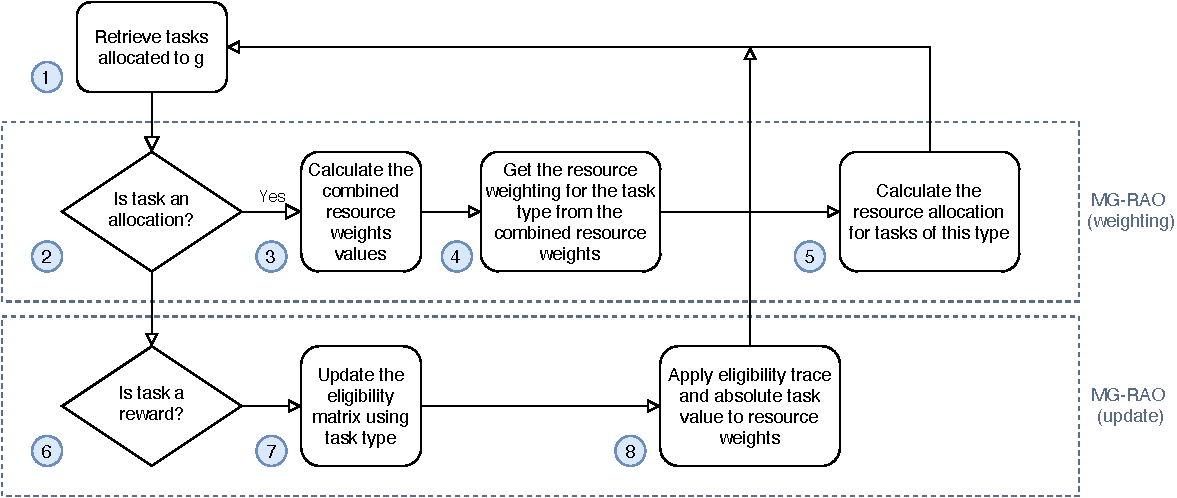
\includegraphics[width=0.8\linewidth, trim={55pt 0pt 55pt 0pt, clip}]{mgrao-simplified}
	\caption{\textbf{Simplified \acronymMGRAO{}{} flowchart}. The diagram shows the decision-making and actions taken by an agent using the \acronymMGRAO{}{}  algorithm. This is a combination of two sub-algorithms, \acronymMGRAO{}{}(weighting), that returns the amount of the agents resources that are allocated to completing the requested task type, and  \acronymMGRAO{}{}(update), that updates its resource weightings from rewards for previous atomic task completions.}
	\label{fig:mgrao-simplified}
\end{figure}
